\documentclass[12pt,notitlepage]{report}
\usepackage[french,english]{babel}
\usepackage[utf8]{inputenc}
\usepackage[
	vmargin = 2cm,
	hmargin = 2.5cm
	]{geometry}
\usepackage[
	defernumbers=true,
	backend=biber,
	style=numeric,
	sorting=nyt
	]{biblatex}
\usepackage[dvipsnames]{xcolor}
\usepackage[T1]{fontenc}
\usepackage[title]{appendix}
\usepackage[most]{tcolorbox}

\usepackage{fancyhdr, listings, minted, verbatim, indentfirst, underscore}
\usepackage{adjustbox, caption, graphicx, subcaption, threeparttable}
\usepackage{lastpage, longtable, tocloft, xcolor, bookmark}
\usepackage{amsmath, amssymb, amsfonts, mathtools}
\usepackage{mathptmx, lmodern}
\usepackage{hyperref, url}
\usepackage{titlesec, notoccite}
\usepackage{tocloft}

% "csquotes should be loaded after fvextra to avoid a warning from the lineno package"
% but in this case the culprit is the "minted" package
\usepackage{csquotes}

%----------------------------------------------------------------------------------
%									  COMMANDES
%----------------------------------------------------------------------------------
\DeclarePairedDelimiter\abs{\lvert}{\rvert}%
\DeclarePairedDelimiter\norm{\lVert}{\rVert}%

\usemintedstyle{fruity}
\definecolor{bg}{HTML}{282828}

\setlength{\headheight}{15.35403pt}
\setlength{\parskip}{0.5em}

\setcounter{secnumdepth}{3}
\counterwithout{table}{chapter}
\counterwithout{equation}{chapter}

\newlistof{links}{lks}{Liste des liens}
\newcommand\externallink[2]{%
\refstepcounter{links}%
\footnote{#1\url{#2}}%
\addcontentsline{lks}{links}{%
\protect\numberline{\thelinks}%
\protect{\url{#2}}}%
}

\hypersetup{
	colorlinks=true,
	linkcolor=blue,
	filecolor=magenta,      
	urlcolor=blue,
	citecolor=darkgray,
	pdftitle={Rapport de stage}
}

\AtEveryBibitem{%
  \clearfield{note}%
}

\newcommand\NB[1][0.3]{N\kern-#1em{B}}

%%Création commande pour insérer image avec nom d figure directement
%\newcommand{nomDeTaCommande}[nombreArguments]{CodeLaTeX}
%\insertImage[position]{image_path}{scale}{Titre_figure}{label}
\newcommand{\insertImage}[5][center]{
	\begin{#1}
		\includegraphics[scale=#3]{#2}
		\captionof{figure}{#4}
		\label{#5}
	\end{#1}
	}
	
	%%Création d'une nouvelle commande pour faire référence à une Figure
	%Exemple : \appelFigure{schema} donne : Figure 1 (en italique)
	\newcommand{\appelFigure}[1]{
		\textit{Figure \ref{#1}}
		}
		
		%%Création d'une nouvelle commande pour créer une barre horizontale
		\newcommand{\HRule}{\rule{\linewidth}{0.5mm}}
		
		\renewcommand{\contentsname}{Table of Contents}
		
		\DeclareMathOperator*{\argmin}{arg\,min}
		\DeclareMathOperator*{\argmax}{arg\,max}
		
		%----------------------------------------------------------------------------------
		%									INITIALISATIONS
		%----------------------------------------------------------------------------------
		\hbadness 11000
		\vbadness 11000
		\interlinepenalty 10000
		
		\title{{\huge \bfseries Pré-traitement et analyse de données génomiques à l'aide d'outils de fouille de données}\\[0.2cm]}
		\author{Théo \textsc{FIGINI}\\M2 Computer Science\\Academic year 2024-2025}
		\date{June, 20\textsuperscript{th} 2025}
		\makeatletter
		\setcounter{chapter}{0}
		
		\pagestyle{fancyplain}
		\fancyhf{}
		\lhead{}
		\rhead{\leftmark}
		\cfoot{Page \thepage /\pageref{LastPage}}
		\renewcommand{\headrulewidth}{0.5pt}
		\renewcommand{\footrulewidth}{0.5pt}
		\renewcommand{\plainheadrulewidth}{0.5pt}
		\renewcommand{\plainfootrulewidth}{0.5pt}
		\renewcommand\labelitemi{--}
		\renewcommand\topfraction{.9}
		\renewcommand\textfraction{0.35}
		\renewcommand\floatpagefraction{0.8}

		\newcommand{\subsubsubsection}[1]{\paragraph{#1}\mbox{}\\}
		
		\counterwithout{figure}{chapter}

		\addbibresource{biblio.bib}
		\DeclareBibliographyCategory{cited}
		\AtEveryCitekey{\addtocategory{cited}{\thefield{entrykey}}}

\begin{document}

\titleformat{\chapter}{\normalfont\large\bfseries}{\thechapter}{20pt}{}
\titleformat{\section}{\normalfont\large\bfseries}{\thesection}{1em}{}
\titleformat{\subsection}{\normalfont\normalsize\bfseries}{\thesubsection}{1em}{}

\titlespacing*{\chapter}{0pt}{-10pt}{25pt}

\begin{titlepage}
	\begin{center}
		
\includegraphics[scale=1.80]{../images/logo_ufr_sen.png} \\[2cm]
		\hspace{2cm}

		\HRule \\[0.4cm]
		\@title
		\HRule \\[1cm]

		\@author \\ [1.5cm]

		{\large Organisme d'accueil~: \textsl{Université des Antilles}} \\[1.5cm]

		\begin{minipage}{0.7\textwidth}
			\begin{center}
				Enseignant~: \\
				\hspace{0.2cm}  XX \textsc{XX}
			\end{center}
		\end{minipage}\\[3cm]

		\@date
	\end{center}
\end{titlepage}


\chapter*{Acknowledgements}
\label{chap:acknowledgements}

I would like to express my heartfelt gratitude to all those who have supported me throughout this project. First and foremost,
I would like to thank my tutor, Dr. \textbf{Wilfried SEGRETIER}, for his invaluable guidance and support during my internship.

I also extend my thanks to Dr. \textbf{Erick STATTNER}, Dr. \textbf{Stephane CHOLET}, and Dr. \textbf{David COUVIN} for their
assistance and for providing me with the additional resources I needed to complete this project.

I would also like to thank my fellow students for their collaboration and support during this project.

Finally, I would like to express my gratitude to my family and friends for their unwavering support and encouragement throughout this journey.

\renewcommand{\thefigure}{\arabic{figure}}
\setcounter{figure}{0}

\pagenumbering{arabic}
\tableofcontents
\addtocontents{toc}{\cftpagenumbersoff{subsec}}

\addcontentsline{toc}{chapter}{abstract}

\hspace{0pt}
\vfill
\begin{otherlanguage}{french}
	\begin{abstract}
		\begin{otherlanguage}{french}
			La tuberculose (TB), causée par Mycobacterium tuberculosis, reste l'une des maladies infectieuses les plus meurtrières
			dans le monde. Comprendre les différentes souches est essentiel pour améliorer les traitements et les stratégies de lutte.
			Ce projet vise à identifier les souches de TB à partir de données de séquençage du génome complet. Nous avons exploré
			des méthodes de regroupement non supervisées et développé des modèles de classification à l'aide de réseaux de neurones
			convolutifs (CNN). Des techniques comme les autoencodeurs et l'augmentation de données ont été utilisées pour améliorer
			les performances. Bien que les résultats soient encore préliminaires, ils montrent un potentiel pour différencier les
			souches de TB selon leurs profils génomiques, ouvrant la voie à des outils de diagnostic plus précis.
		\end{otherlanguage}
	\end{abstract}
\end{otherlanguage}

\begin{abstract}
	Tuberculosis (TB), caused by Mycobacterium tuberculosis, remains one of the\\world's most deadly infectious diseases. Understanding
	its different strain types is vital for improving treatment and control efforts. This project focuses on identifying TB strains
	using whole genome sequencing data. We explored unsupervised clustering methods and developed classification models using
	convolutional neural networks (CNNs). Techniques such as autoencoders and data augmentation were also applied to enhance
	performance. While the results are preliminary, they demonstrate potential for differentiating TB strains based on genomic
	patterns, laying the groundwork for more refined diagnostic tools.
\end{abstract}
\vfill
\hspace{0pt}
\chapter*{Introduction}

Introduction
\chapter{Related Work}
\label{chap:related-work}

Genomics is a field that has been growing rapidly in the past few years. The advent of high-throughput
sequencing technologies has made it possible to sequence the entire genome of an organism in a matter
of days. This has led to an explosion of data, with the number of sequenced genomes increasing exponentially.
This has created a need for new tools and algorithms to analyze this data. In this chapter, we review
some of the existing tools and algorithms for analyzing genomic data. We also discuss some of the techniques
we used in our project.

\section{Genomic data analysis}
\label{sec:genomic-data-analysis}

\subsection*{Random forests}
\label{subsec:random-forests}

Another method that has been used for genomic data analysis is random forests (RF) \cite{Chen-Ishwaran-2012}.
This method is based on the idea of ensemble learning, where multiple decision trees are trained on different
subsets of the data and then combined to make a final prediction.

\subsection*{AI applications in genomic analysis}
\label{sec:ai-applications-in-genomic-analysis}

Many researchers have used AI techniques to analyze genomic data. For example, \cite{Caudai-et-al-2021} reviews
different AI techniques that have been used for genomic data analysis, including CNNs, autoencoders, etc.

More recently, the authors of \cite{Zhou-et-al-2024} designed a tool based on multiple LLM backends for multi-omics
analysis with minimal human intervention.

\section{DBSCAN and HDBSCAN}
\label{sec:principle_dbscan_hdbscan}

\subsection*{DBSCAN}
\label{subsec:dbscan}

DBSCAN works by defining a neighborhood around each point based on a distance metric (usually Euclidean distance) and a
minimum number of points required to form a dense region. The algorithm proceeds as follows:

\begin{enumerate}
	\item For each point in the dataset, find its neighbors within a specified radius $\varepsilon$.
	\item If the number of neighbors is greater than or equal to the minimum number of points, a new cluster is formed.
	\item The algorithm recursively expands the cluster by including all points that are reachable from the initial point.
	\item Points that do not belong to any cluster are classified as noise.
\end{enumerate}

\subsection*{HDBSCAN}
\label{subsec:hdbscan}

HDBSCAN builds on the principles of DBSCAN by introducing a hierarchical clustering approach. It is more robust to varying
densities and can identify clusters of different shapes and sizes. The algorithm works as follows:

\begin{enumerate}
	\item Compute the mutual reachability distance between points, which takes into account the distance to the nearest neighbor.
	\item Build a minimum spanning tree (MST) based on the mutual reachability distances.
	\item Extract clusters from the MST by varying the density threshold, resulting in a hierarchy of clusters.
	\item Assign points to clusters based on their membership in the hierarchy, allowing for flexible clustering.
\end{enumerate}

\section{Introduction to CNNs}
\label{sec:intro_cnn}

The fundamental idea behind \textbf{Convolutional Neural Networks (CNNs)} was introduced by Kunihiko Fukushima\textsuperscript{\cite{Fukushima-1987}}
in 1980 and later popularized by Yann LeCun in the 1990s with the LeNet architecture\textsuperscript{\cite{Lecun-et-al-1998}}. CNNs are a class of
deep learning models specifically designed for processing structured grid data, such as images. They are particularly effective for
tasks like image classification, object detection, and segmentation.

CNNs work by applying convolutional filters to the input data, which allows them to learn spatial hierarchies of features.
It shares some similarities with the more conventional neural networks, but there is at least two different types
of layers that are specific to CNNs:

\begin{itemize}
	\item \textbf{Convolutional layers}: These layers apply convolutional filters to the input data, extracting local features
	      that are invariant to translation. The filters slide over the input data, computing dot products and producing feature maps.
	\item \textbf{Pooling layers}: These layers downsample the feature maps, reducing their spatial dimensions while retaining important
	      information. Common pooling operations include max pooling and average pooling.
\end{itemize}

The architecture of a CNN typically consists of multiple convolutional and pooling layers followed by fully connected layers.
The convolutional layers learn to extract features from the input data, while the fully connected layers perform the final classification
or regression task. The training process involves optimizing the weights of the filters and fully connected layers using backpropagation
and a loss function, such as cross-entropy for classification tasks.

\section{K-fold cross validation}
\label{sec:k_fold_cross_validation}

K-fold cross validation is a specific type of cross validation where the dataset is divided into $k$ equally sized folds. The model is trained
on $k-1$ folds and tested on the remaining fold, and this process is repeated for each fold. The final performance is averaged over all folds
to obtain a more reliable estimate of the model's performance. The graphical representation of K-fold cross validation is shown in Figure~\ref{fig:k_fold}.

\begin{figure}[htbp]
	\centering
	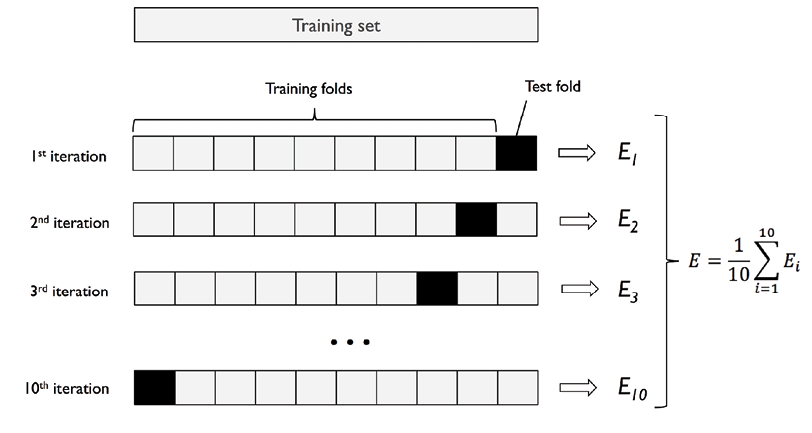
\includegraphics[width=0.8\textwidth]{../imgs/kfold.png}
	\caption{How K-fold cross validation works.\textsuperscript{\cite{Raschka-Mirjalili-2017}}}
	\label{fig:k_fold}
\end{figure}

\subsubsection{Stratified K-fold cross validation}
\label{subsec:stratified_k_fold_cross_validation}

Stratified K-fold cross validation is a variation of K-fold cross validation that ensures that each fold has the same proportion of samples
from each class. This is particularly useful for imbalanced datasets, as it ensures that each fold has a representative sample of each class.
Even if this method is recommended for imbalanced datasets, we did not have enough time to implement it, so we used the standard K-fold cross
validation.

\section{SMOTE}
\label{sec:smote}

Data augmentation is a technique used to artificially increase the size of a dataset by applying various transformations to the existing data.
This can help improve the model's performance by providing more diverse training samples and reducing overfitting. In our project, we used SMOTE
(Synthetic Minority Over-sampling Technique) to generate synthetic samples for the minority classes in our dataset.

SMOTE works by creating new samples by interpolating between existing samples in the feature space. It generates synthetic samples by selecting
a minority class sample, finding its nearest neighbors, and creating new samples by interpolating between the selected sample and its neighbors.
This helps to balance the dataset by increasing the number of samples in the minority classes, which can improve the model's performance on those
classes.

New samples are generated by taking a random sample from the minority class and finding its nearest neighbors in the feature space. The new sample
is then created by interpolating between the selected sample and its neighbors, as shown in Figure~\ref{fig:smote}. It uses the following formula:

\begin{equation}
	x_{new} = x_{i} + \lambda (x_{j} - x_{i})
\end{equation}

Where $x_{new}$ is the new sample, $x_{i}$ is the selected sample, $x_{j}$ is one of its nearest neighbors, and $\lambda$ is a random number
between 0 and 1. This process is repeated until the desired number of samples is generated for the minority class.

\begin{figure}[htbp!]
	\centering
	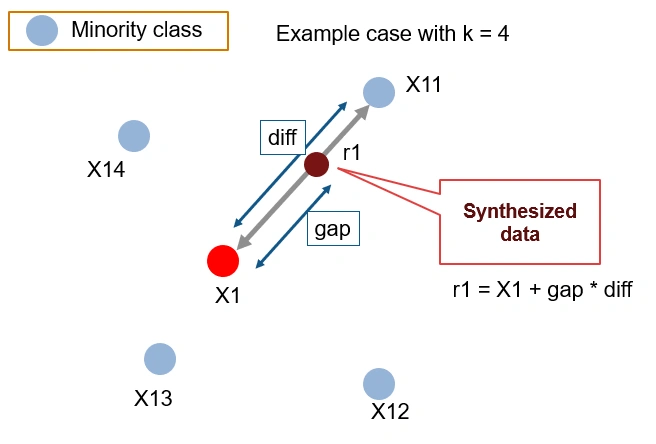
\includegraphics[width=0.6\textwidth]{../imgs/smote.png}
	\caption{Illustration of the SMOTE algorithm.\textsuperscript{\cite{analyticsvidhya-2020}}}
	\label{fig:smote}
\end{figure}
\chapter{Problem Statement}
\label{chap:problem_statement}

\section{Context}
\label{sec:context}

\section{Work Environment}
\label{sec:work_environment}

This project was done within the framework of the Master 2 Computer Science program at the
\textbf{Laboratoire de Mathématiques Informatique et Applications (LAMIA)} of the \textbf{Université des Antilles}.
The following tools and technologies were used to develop the algorithms and document the project:

\begin{itemize}
	\item \textbf{Python}: a programming language widely used in scientific computing, data analysis, and machine learning.
	\item \textbf{GitHub}: a version control platform for managing the source code.
	\item \textbf{Jupyter Notebook}: an interactive environment for writing and executing Python code, ideal for data analysis and
	      visualization.
	\item \textbf{sklearn}: a Python library for machine learning that provides various algorithms and tools for data preprocessing,
	      model selection, and evaluation.
	\item \LaTeX : a typesetting system used for writing technical and scientific documents.
	\item A personal computer running Windows 11 with a \textbf{Ryzen 7 6800H} processor and \textbf{32 GB} of RAM.
\end{itemize}

\section{Objectives}
\label{sec:objectives}

\chapter{Genomic data}
\label{chap:genomic_data}

Genomic data refers to the information contained in the DNA of an organism, which includes the sequences of nucleotides (A, T, C, G).
These are gathered through various methods, such as DNA sequencing, and can be used to study the genetic makeup of organisms,
identify genetic variations, and understand the relationships between different species. The Institut Pasteur has a large collection
of genomic data, including the genomes of various strains of Tuberculosis (TB), which is a major public health concern worldwide.

\section{The FASTA format}
\label{sec:fasta_format}

The FASTA format is a text-based format for representing nucleotide or protein sequences. It is widely used in bioinformatics
to store and exchange sequence data. A FASTA file consists of one or more sequences, each represented by a header line starting with
a greater-than symbol (\texttt{>}), followed by the sequence itself on the next line. The header line can contain additional
information about the sequence, such as its identifier, description, or source. An example of a FASTA file is shown in
Figure~\ref{fig:fasta_example}.

\begin{center}
	\begin{figure}[htbp]
		\begin{BVerbatim}
			>sequence_id
			ATCGATCGATCGATCGATCGATCGATCG
			>another_sequence_id
			GCTAGCTAGCTAGCTAGCTAGCTAGCTA
		\end{BVerbatim}
		\caption{Example of a FASTA file containing two sequences.}
		\label{fig:fasta_example}
	\end{figure}
\end{center}

The FASTA format is simple and easy to read, making it suitable for storing large amounts of sequence data. It is also compatible with
many bioinformatics tools and software, allowing for easy analysis and manipulation of sequence data.

\chapter{Clustering genomic data}
\label{chap:clustering_genomic_data}

\section{Introduction to K-means}
\label{sec:intro_kmeans}

K-means clustering is a widely used unsupervised learning algorithm for partitioning a dataset into $k$ distinct clusters.
It works by iinitializing $k$ cluster centers, then iteratively assigning data points to the nearest cluster center and
updating the centers based on the distances to the assigned points (usually using Euclidean distance). The algorithm
continues until the cluster centers stabilize or a maximum number of iterations is reached.

Results can vary based on the initial choice of cluster centers, which can lead to different clustering outcomes.
The quality of clusters is typically evaluated using at least two criteria:

\begin{itemize}
	\item \textbf{Intra-cluster variance} : the average distance between points within the same cluster.
	\item \textbf{Inter-cluster variance} : the average distance between centers of different clusters.
\end{itemize}

\subsection{K-means Algorithm}
\label{subsec:kmeans_algorithm}

The K-means algorithm consists of the following steps:
\begin{enumerate}
	\item Initialize $k$ cluster centers randomly.
	\item Assign each data point to the nearest cluster center.
	\item Update the cluster centers by calculating the mean of the points assigned to each cluster.
	\item Repeat steps 2 and 3 until convergence (i.e., when cluster centers do not change significantly).
	\item Optionally, evaluate the clustering quality using metrics like inertia or silhouette score.
\end{enumerate}

\section{Silhouette Score}
\label{subsec:silhouette_score}

The silhouette score is a metric used to evaluate the quality of clustering. It measures how similar an object
is to its own cluster compared to other clusters. The silhouette score is calculated for each data point and
ranges from -1 to 1. The formula for the silhouette score of a point $i$ is:

\begin{equation}
	s(i) = \frac{b(i) - a(i)}{\max(a(i), b(i))}
\end{equation}

Where $a(i)$ is the average distance from point $i$ to all other points in the same cluster, and $b(i)$ is the
average distance from point $i$ to all points in the nearest cluster. A higher silhouette score indicates better
clustering quality.

\section{Principal Component Analysis (PCA)}
\label{subsec:pca}

Principal Component Analysis (PCA) is a dimensionality reduction technique that transforms a dataset into a new coordinate system,
where the axes (principal components) are ordered by the amount of variance they capture from the data. It was first introduced by
\textbf{Karl Pearson} in 1901\textsuperscript{\cite{Pearson-1901}} and later popularized by \textbf{Harold Hotelling} in
1933\textsuperscript{\cite{Hotelling-1933}}. PCA is widely used in data analysis, PCA is particularly useful for reducing the
dimensionality of large datasets while preserving as much variance as possible. The steps involved in PCA are:

\begin{enumerate}
	\item \textbf{Standardize the data}: Center the data by subtracting the mean and scaling it to unit variance.
	\item \textbf{Compute the covariance matrix}: Calculate the covariance matrix of the standardized data.
	\item \textbf{Compute the eigenvalues and eigenvectors}: Find the eigenvalues and eigenvectors of the covariance matrix.
	\item \textbf{Sort the eigenvalues and eigenvectors}: Sort the eigenvalues in descending order and arrange the corresponding
	      eigenvectors accordingly.
	\item \textbf{Select the top $k$ eigenvectors}: Choose the top $k$ eigenvectors corresponding to the largest eigenvalues, where $k$ is
	      the desired number of dimensions to retain.
	\item \textbf{Transform the data}: Project the original data onto the new coordinate system defined by the selected eigenvectors.
\end{enumerate}

Note: an eigenvector or characteristic vector is a vector that does not change direction during a linear transformation,
but may change in magnitude. The eigenvalue is the factor by which the eigenvector is scaled during the transformation.

In this project, we use the integrated PCA implementation from the \textit{sklearn} library, which provides a convenient way to perform PCA
on datasets.

\section{Preprocessing Genomic Data}
\label{sec:preprocessing_genomic_data}

Our data is a collection of Tuberculosis (TB) genomes, where each file contains the proteins and their respective
nucleotide sequences in FASTA format, for a total of 7057 files.
TODO: parler de l'institut Pasteur?
The goal is to cluster these genomes based on their protein sequences and find ways to distinguish between different
TB strains.

We started by creating a dataset containing the number of times each protein appears in each genome. This was done by
parsing the FASTA files and counting the occurrences of each protein sequence, we then removed the outliers, namely
"hypothetical proteins" and "putative proteins", which are not well characterized and do not provide useful information
for clustering. The resulting dataset is a CSV file of 7057 columns plus 1 column for the protein names and 2732 rows
plus 1 row for the header.

Considering the size of the dataset, we used Principal Component Analysis (PCA) set to 95\% variance to reduce the dimensionality
of the data while preserving as much variance as possible. PCA is a technique that transforms the data into a new coordinate
system, where the first principal component captures the maximum variance, the second captures the second maximum variance,
and so on.

We then calculated the silhouette score for different values of $k$, ranging from 2 to 10, to determine the optimal number
of clusters. The silhouette score was calculated using the `silhouette_score` function from the `sklearn.metrics` module,
which takes the data and the cluster labels as input. The optimal number of clusters is the one that maximizes the silhouette
score.

\subsection{First Results}
\label{subsec:first_results}

The initial results showed that the silhouette score was highest for $k=9$, indicating that this was the optimal number of clusters.
However, the clusters were not well separated or some points are alone in their cluster, as seen in Figure {TODO:figure:clusters_k9}.
Which suggests that the data may not be well suited for clustering with K-means, or that the features used for clustering are not
informative enough.

TODO: figure clusters_k9

We also tried without applying PCA but achieved similar results, we also observed a fewer points than expected as seen in
Figure {TODO:figure:clusters_k9_no_pca}, after reviewing the data, we found that there is significant overlap between the points.

TODO: figure clusters_k9_no_pca

So we switched to 3D visualization to better understand the clusters,

\section{New Approach using DBSCAN and HDBSCAN}
\label{subsec:new_approach_dbscan_hdbscan}

To address the limitations of K-means clustering, we explored alternative clustering algorithms, specifically
\textbf{DBSCAN} and \textbf{HDBSCAN}.

DBSCAN (Density-Based Spatial Clustering of Applications with Noise) is a density-based clustering algorithm that
groups points that are close together based on a distance measurement and a minimum number of points. It is particularly
effective for datasets with varying densities and can identify noise points that do not belong to any cluster.

HDBSCAN (Hierarchical Density-Based Spatial Clustering of Applications with Noise) is an extension of DBSCAN that builds
a hierarchy of clusters and allows for more flexible clustering by varying the density threshold. It can also handle varying
cluster shapes and sizes.

\subsection{Principle}
\label{subsec:principle_dbscan_hdbscan}

\subsubsubsection{DBSCAN}
\label{subsubsec:dbscan}

DBSCAN works by defining a neighborhood around each point based on a distance metric (usually Euclidean distance) and a
minimum number of points required to form a dense region. The algorithm proceeds as follows:

\begin{enumerate}
	\item For each point in the dataset, find its neighbors within a specified radius $\varepsilon$.
	\item If the number of neighbors is greater than or equal to the minimum number of points, a new cluster is formed.
	\item The algorithm recursively expands the cluster by including all points that are reachable from the initial point.
	\item Points that do not belong to any cluster are classified as noise.
\end{enumerate}

\subsubsubsection{HDBSCAN}
\label{subsubsec:hdbscan}

HDBSCAN builds on the principles of DBSCAN by introducing a hierarchical clustering approach. It is more robust to varying
densities and can identify clusters of different shapes and sizes. The algorithm works as follows:

\begin{enumerate}
	\item Compute the mutual reachability distance between points, which takes into account the distance to the nearest neighbor.
	\item Build a minimum spanning tree (MST) based on the mutual reachability distances.
	\item Extract clusters from the MST by varying the density threshold, resulting in a hierarchy of clusters.
	\item Assign points to clusters based on their membership in the hierarchy, allowing for flexible clustering.
\end{enumerate}

\subsection{Results}
\label{subsec:results_dbscan_hdbscan}

\section{Trying an autoencoder}
\label{sec:autoencoder}

\chapter{Using CNNs to identify TB Strains}
\label{chap:cnn_tb_strains}

\section{Introduction to CNNs}
\label{sec:intro_cnn}

The fondamental idea behind \textbf{Convolutional Neural Networks (CNNs)} was introduced by Kunihiko Fukushima\textsuperscript{\cite{Fukushima-1987}}
in 1980 and later popularized by Yann LeCun in the 1990s with the LeNet architecture\textsuperscript{\cite{Lecun-et-al-1998}}. CNNs are a class of
deep learning models specifically designed for processing structured grid data, such as images. They are particularly effective for
tasks like image classification, object detection, and segmentation.

CNNs work by applying convolutional filters to the input data, which allows them to learn spatial hierarchies of features.
It shares some similarities with the more conventional neural networks, but there is at least two different types
of layers that are specific to CNNs:

\begin{itemize}
	\item \textbf{Convolutional layers}: These layers apply convolutional filters to the input data, extracting local features
	      that are invariant to translation. The filters slide over the input data, computing dot products and producing feature maps.
	\item \textbf{Pooling layers}: These layers downsample the feature maps, reducing their spatial dimensions while retaining important
	      information. Common pooling operations include max pooling and average pooling.
\end{itemize}

The architecture of a CNN typically consists of multiple convolutional and pooling layers followed by fully connected layers.
The convolutional layers learn to extract features from the input data, while the fully connected layers perform the final classification
or regression task. The training process involves optimizing the weights of the filters and fully connected layers using backpropagation
and a loss function, such as cross-entropy for classification tasks.

\section{Building the dataset}
\label{sec:building_dataset}

For this experiment, each genome was converted into an image where each pixel is determined by a combination of three metrics of following
metrics:

\begin{itemize}
	\item \textbf{Chargaff}
	\item \textbf{Composition}
	\item \textbf{Diversity}
	\item \textbf{Skew}
	\item \textbf{Nuclescore}
\end{itemize}

We get ten combinations of these metrics, each represented by a different color channel in the image. We applied this conversion at different
resolutions, from 4px (2x2) to 100px (10x10), the resulting images put into their corresponding class based on the strain they belong to. We
have the following classes:

\begin{itemize}
	\item \textbf{M} with 185 samples.
	\item \textbf{East Asian} with 1651 samples.
	\item \textbf{East-African Indian} with 267 samples.
	\item \textbf{Euro-American} with 4409 samples.
	\item \textbf{Indo-Oceanic} with 259 samples.
\end{itemize}


\subsection{Initial testing}
\label{subsec:initial_testing}

The resulting dataset is highly imbalanced, with some classes having significantly more samples than others. This can lead to biased models
that perform poorly on minority classes. We decided to train our CNN on the dataset as-is, without any preprocessing or balancing techniques,
to see how it performs on the imbalanced dataset.

\section{Mitigating class imbalance}
\label{sec:mitigating_class_imbalance}

We have multiple ways of addressing the class imbalance issue in our dataset, including:
\begin{itemize}
	\item Cross validation
	\item Under-sampling
	\item Data augmentation
	\item Combining under-sampling and data augmentation
\end{itemize}

We will explore each of these techniques in the following sections and compare the results to see which one yields the best performance.

\subsection{Cross validation}
\label{subsec:cross_validation}

Cross validation is a technique used to evaluate the performance of a model by splitting the dataset into multiple subsets, or folds.
The model is trained on a subset of the data and tested on the remaining data, and this process is repeated for each fold.
This allows for a more robust evaluation of the model's performance, as it reduces the risk of overfitting to a specific subset of the data.
\subsubsubsection{K-fold cross validation}
\label{subsubsec:k_fold_cross_validation}

K-fold cross validation is a specific type of cross validation where the dataset is divided into $k$ equally sized folds. The model is trained
on $k-1$ folds and tested on the remaining fold, and this process is repeated for each fold. The final performance is averaged over all folds
to obtain a more reliable estimate of the model's performance. The graphical representation of K-fold cross validation is shown in Figure~\ref{fig:k_fold}.

\begin{figure}[htbp]
	\centering
	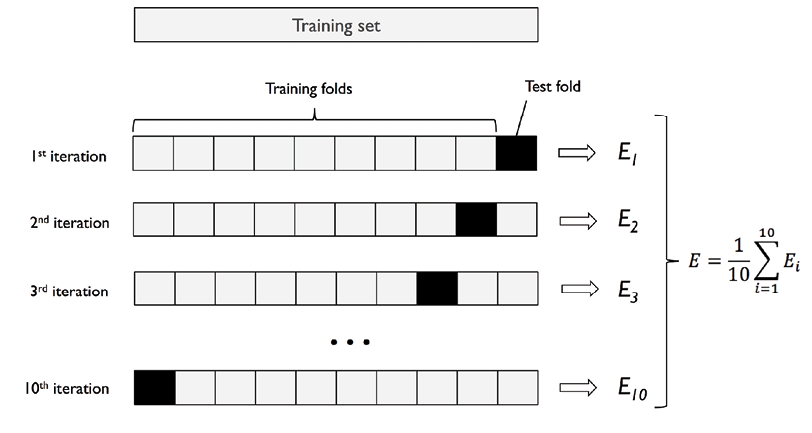
\includegraphics[width=0.8\textwidth]{../imgs/kfold.png}
	\caption{How K-fold cross validation works.\textsuperscript{\cite{Raschka-Mirjalili-2017}}}
	\label{fig:k_fold}
\end{figure}


\subsubsubsection{Stratified K-fold cross validation}
\label{subsubsec:stratified_k_fold_cross_validation}

Stratified K-fold cross validation is a variation of K-fold cross validation that ensures that each fold has the same proportion of samples
from each class. This is particularly useful for imbalanced datasets, as it ensures that each fold has a representative sample of each class.
Even if this method is recommended for imbalanced datasets, we did not have enough time to implement it, so we used the standard K-fold cross
validation.

\subsubsubsection{Remaking the dataset}
\label{subsubsec:remaking_dataset}

During our testing, we realized that we were testing our model with images the model was trained on, which is not a good practice. We decided to
split our dataset into a training set and a test set, with 90\% of the samples in the training set and 10\% in the test set. The files are separated
into two folders to avoid any overlap between the training and test sets.

\subsection{Under-sampling}
\label{subsec:under_sampling}


\subsection{Data augmentation}
\label{subsec:data_augmentation}

\subsubsubsection{SMOTE}
\label{subsubsec:smote}

Data augmentation is a technique used to artificially increase the size of a dataset by applying various transformations to the existing data.
This can help improve the model's performance by providing more diverse training samples and reducing overfitting. in our project, we used SMOTE
(Synthetic Minority Over-sampling Technique) to generate synthetic samples for the minority classes in our dataset.

SMOTE works by creating new samples by interpolating between existing samples in the feature space. It generates synthetic samples by selecting
a minority class sample, finding its nearest neighbors, and creating new samples by interpolating between the selected sample and its neighbors.
This helps to balance the dataset by increasing the number of samples in the minority classes, which can improve the model's performance on those
classes.

New samples are generated by taking a random sample from the minority class and finding its nearest neighbors in the feature space. The new sample
is then created by interpolating between the selected sample and its neighbors, as shown in Figure~\ref{fig:smote}. It uses the following formula:

\begin{equation}
	x_{new} = x_{i} + \lambda (x_{j} - x_{i})
\end{equation}

where $x_{new}$ is the new sample, $x_{i}$ is the selected sample, $x_{j}$ is one of its nearest neighbors, and $\lambda$ is a random number
between 0 and 1. This process is repeated until the desired number of samples is generated for the minority class.

\begin{figure}[htbp!]
	\centering
	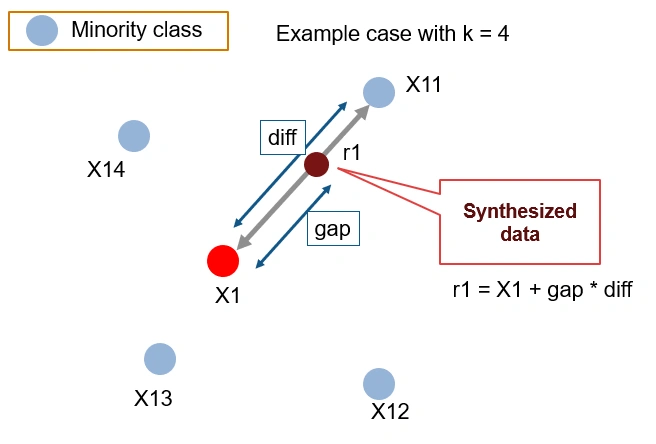
\includegraphics[width=0.7\textwidth]{../imgs/smote.png}
	\caption{Illustration of the SMOTE algorithm.\textsuperscript{\cite{analyticsvidhya-2020}}}
	\label{fig:smote}
\end{figure}

\subsubsubsection{Results}
\label{subsubsec:results_data_augmentation}



\subsection{Combining techniques}
\label{subsec:combining_techniques}

\subsubsubsection{Results}
\label{subsubsec:results_combining_techniques}
\chapter{Conclusion}
\label{chap:conclusion}

During this project, we have explored various techniques for genomic data pre-processing and analysis, focusing on the Mycobacterium tuberculosis (MTB)
genome. We have implemented several methods for data pre-processing and analysis, such as K-means clustering, DBSCAN, HDBSCAN and an autoencoder.
However, we encountered several challenges, particularly with the clustering methods, which did not yield satisfactory results. We theorized that,
either the data was not suitable for clustering due to its high dimensionality, or that they were not prepared correctly.

We also explored the use of Convolutional Neural Networks (CNNs) for image classification, which showed promising results. The images were generated
from the genomic data by applying a combination of three of five metrics to the nucleotide sequences, resulting in ten different combinations of metrics,
each represented by a different color channel in the image. We also created a dataset of mosaic images, combining the images from the ten different
combinations of metrics.

The resulting dataset was highly imbalanced, with a significant number of samples belonging to two of the fives classes,
Euro-American and East-Asian. To address this issue, we applied different techniques such as K-fold cross validation, under-sampling, data augmentation
using SMOTE, and a combination of both under-sampling and data augmentation. The best results were achieved with the data augmentation technique,
which improved the metrics for the Indo-Oceanic class on the individual images, and the East-African Indian class on the mosaic images.

Another behavior we observed was that, despite being the class with the lowest number of samples, the M class always had metrics on par or close to the
majority classes. This suggests that the M class has a specific pattern that is distinct from the other classes, which could be further investigated
in future work.

In conclusion, this project has provided valuable insights into the challenges and opportunities of genomic data pre-processing and analysis.
We have demonstrated the potential of using CNNs for image classification of genomic data, and the importance of addressing class imbalance
in the dataset. I personally learned a lot about the fields of genomics and bioinformatics. This project has been a great opportunity to apply
my knowledge in machine learning and data analysis to a real-world problem.

\begin{appendices}

	\chapter{Additional Figures}
	\label{app:additional_figures}

	% ------ kfold cross validation ------

	\begin{figure}[H]
		\centering
		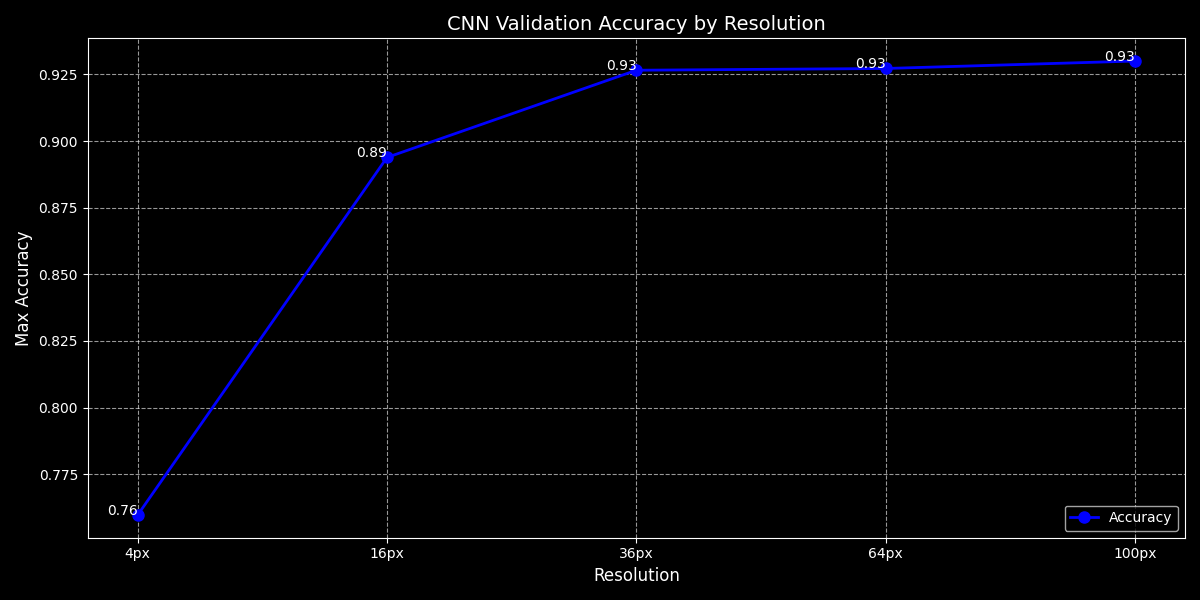
\includegraphics[width=0.65\textwidth]{../imgs/graphs/kfold/cnn_validation_accuracy_kfold_mosaics_line_mask_5_std.png}
		\caption{Graph showing the validation accuracy of the CNN model with k-fold cross validation applied on the mosaic images.}
		\label{fig:kfold_accuracy_mosaic}
	\end{figure}

	\begin{figure}[H]
		\centering
		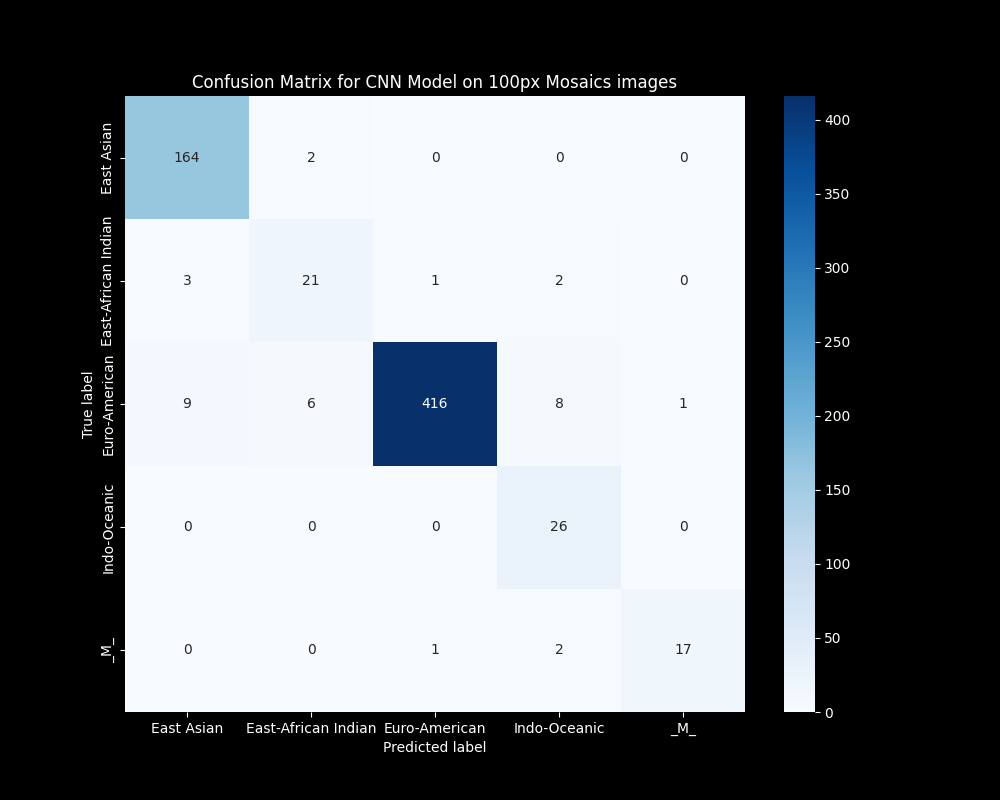
\includegraphics[width=0.65\textwidth]{../imgs/graphs/kfold/cnn_confusion_matrix_kfold_mosaics_100px_mask_5_std.png}
		\caption{Confusion matrix of the CNN model with k-fold cross validation applied on the mosaic images at 100px resolution.}
		\label{fig:kfold_confusion_matrix_mosaic}
	\end{figure}

	% ------ kfold cross validation with under-sampling ------

	\begin{figure}[htbp!]
		\centering
		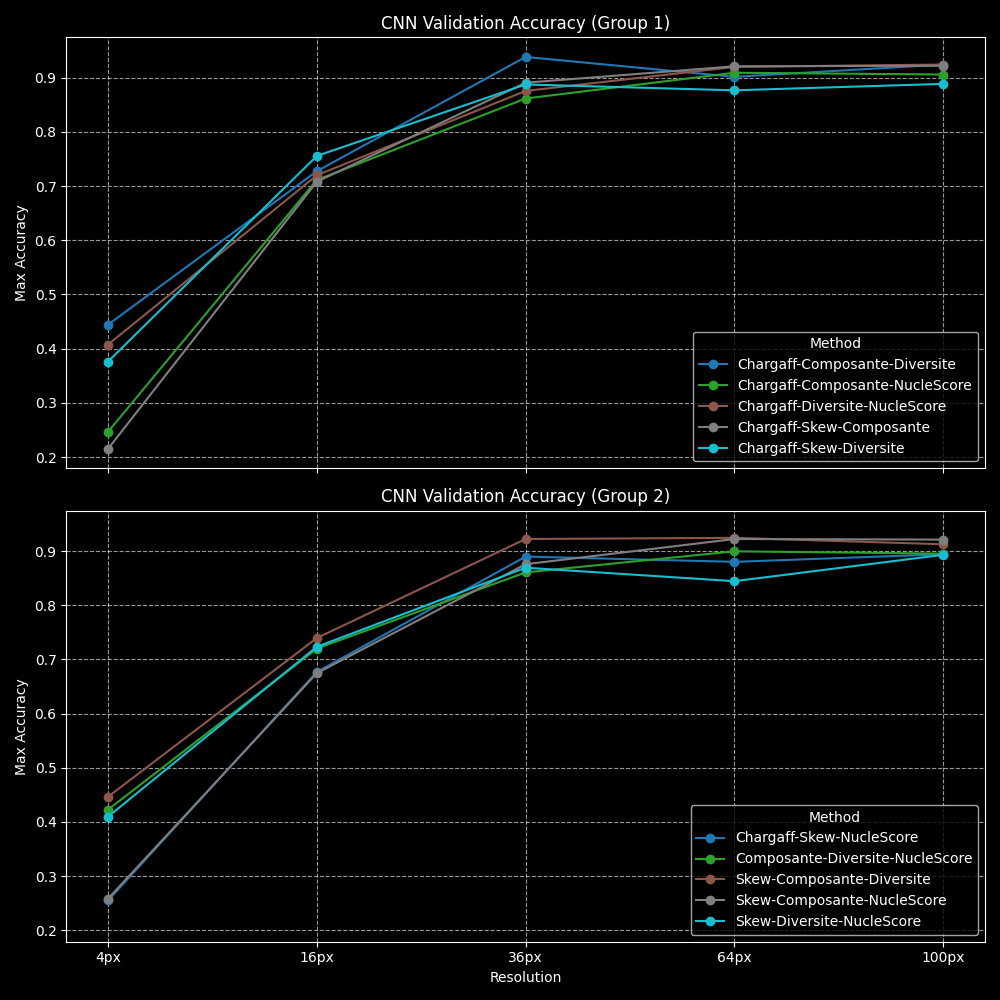
\includegraphics[width=0.7\textwidth]{../imgs/graphs/kfold-undersample/cnn_validation_accuracy_groups_mask_5_kfold_undersample.png}
		\caption{Graph showing the validation accuracy of the CNN model with under-sampling applied on the different methods.}
		\label{fig:under_sampling_accuracy}
	\end{figure}

	\begin{figure}[htbp!]
		\centering
		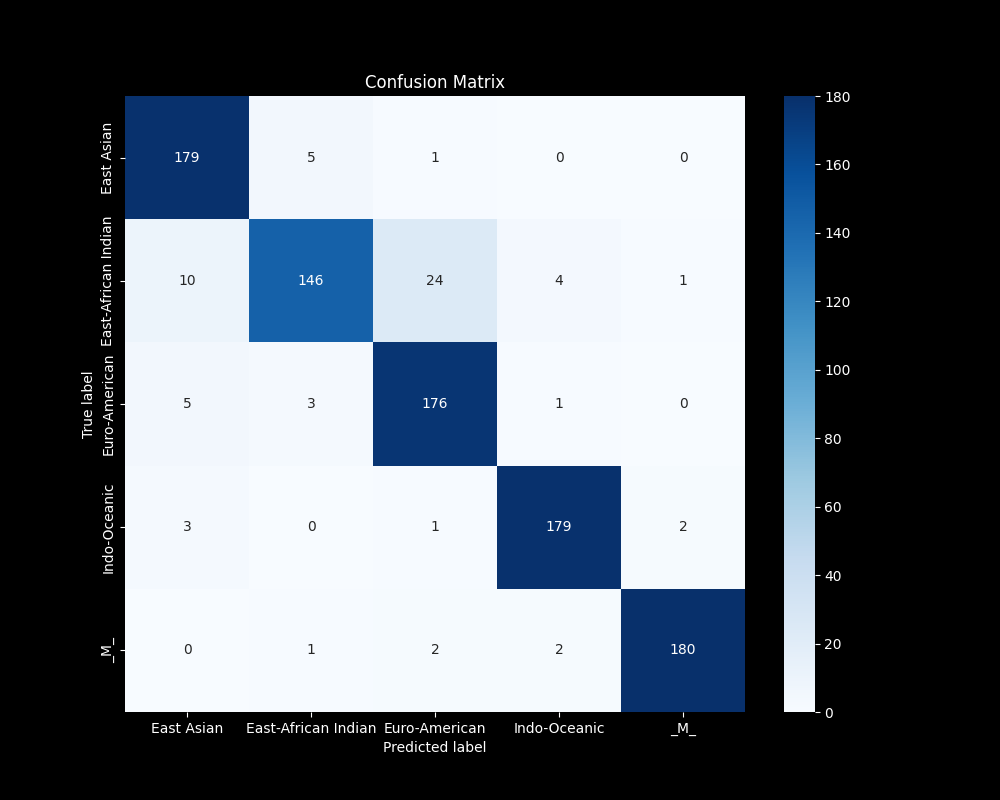
\includegraphics[width=0.7\textwidth]{../imgs/graphs/kfold-undersample/cnn_confusion_matrix_100px_mask_5-kfold_undersample.png}
		\caption{Confusion matrix of the CNN model with under-sampling applied on the images obtained from the Chargaff-Diversity-NucleScore
			combination at 100px resolution.}
		\label{fig:under_sampling_confusion_matrix}
	\end{figure}

	\begin{figure}[htbp!]
		\centering
		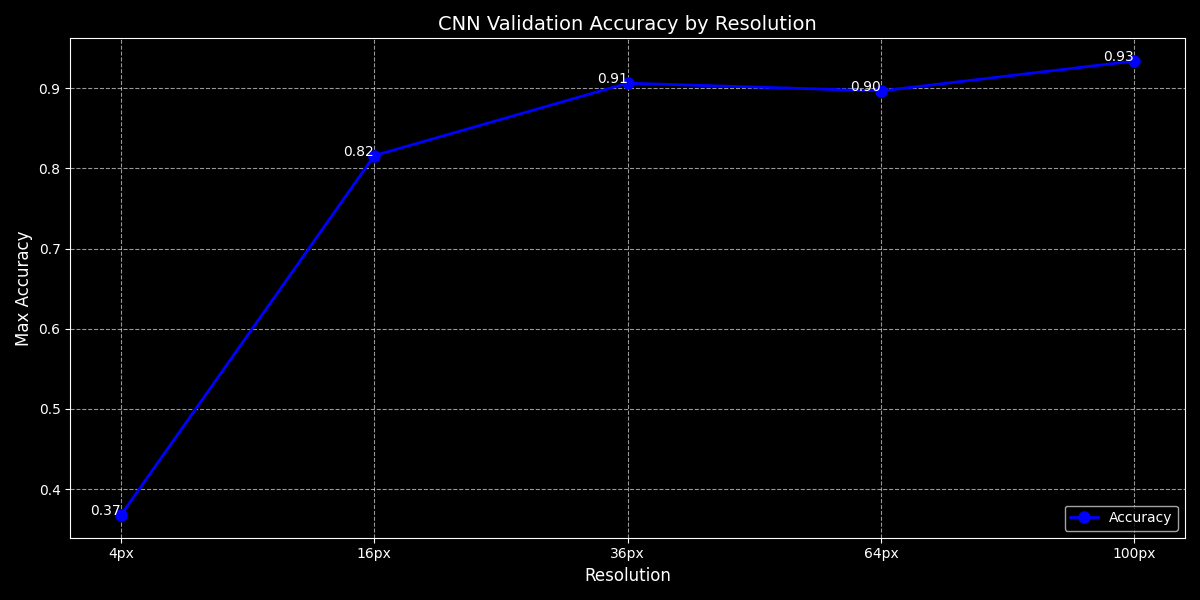
\includegraphics[width=0.7\textwidth]{../imgs/graphs/kfold-undersample/cnn_validation_accuracy_kfold_mosaics_line_mask_5_undersample.png}
		\caption{Graph showing the validation accuracy of the CNN model with under-sampling applied on the mosaic images.}
		\label{fig:under_sampling_mosaic_accuracy}
	\end{figure}

	\begin{figure}[htbp!]
		\centering
		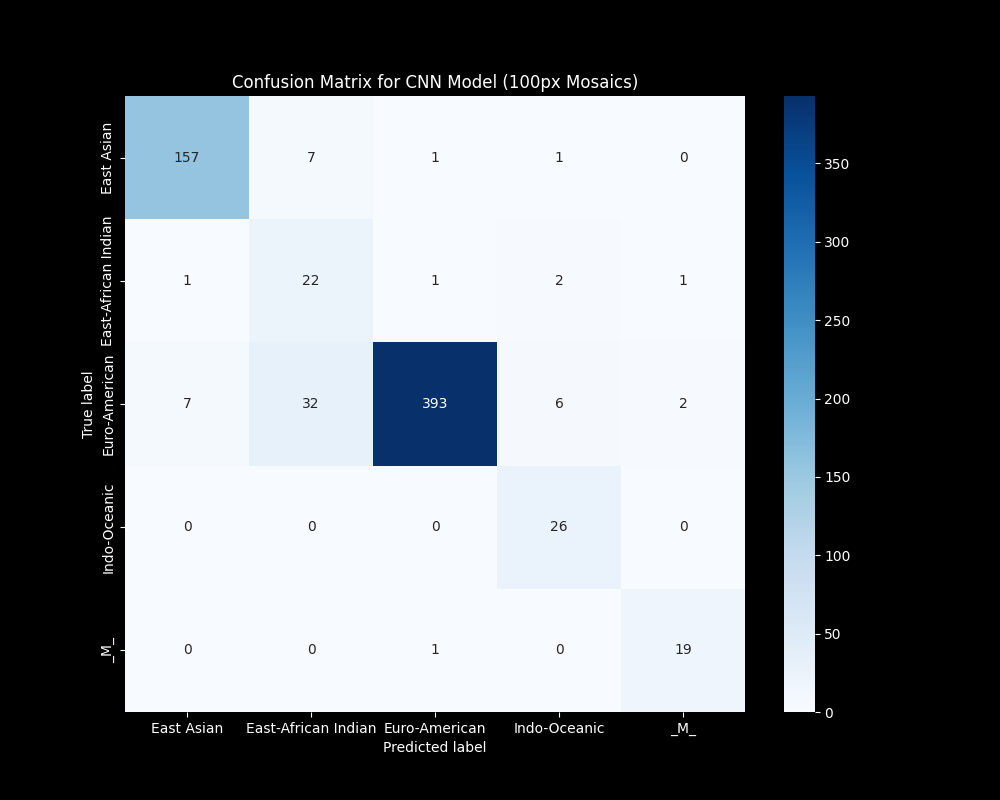
\includegraphics[width=0.7\textwidth]{../imgs/graphs/kfold-undersample/cnn_confusion_matrix_kfold_mosaics_100px_mask_5_undersample.png}
		\caption{Confusion matrix of the CNN model with under-sampling applied on the mosaic images at 100px resolution.}
		\label{fig:under_sampling_mosaic_confusion_matrix}
	\end{figure}

	% ------ kfold cross validation with data augmentation ------

	\begin{figure}[htbp!]
		\centering
		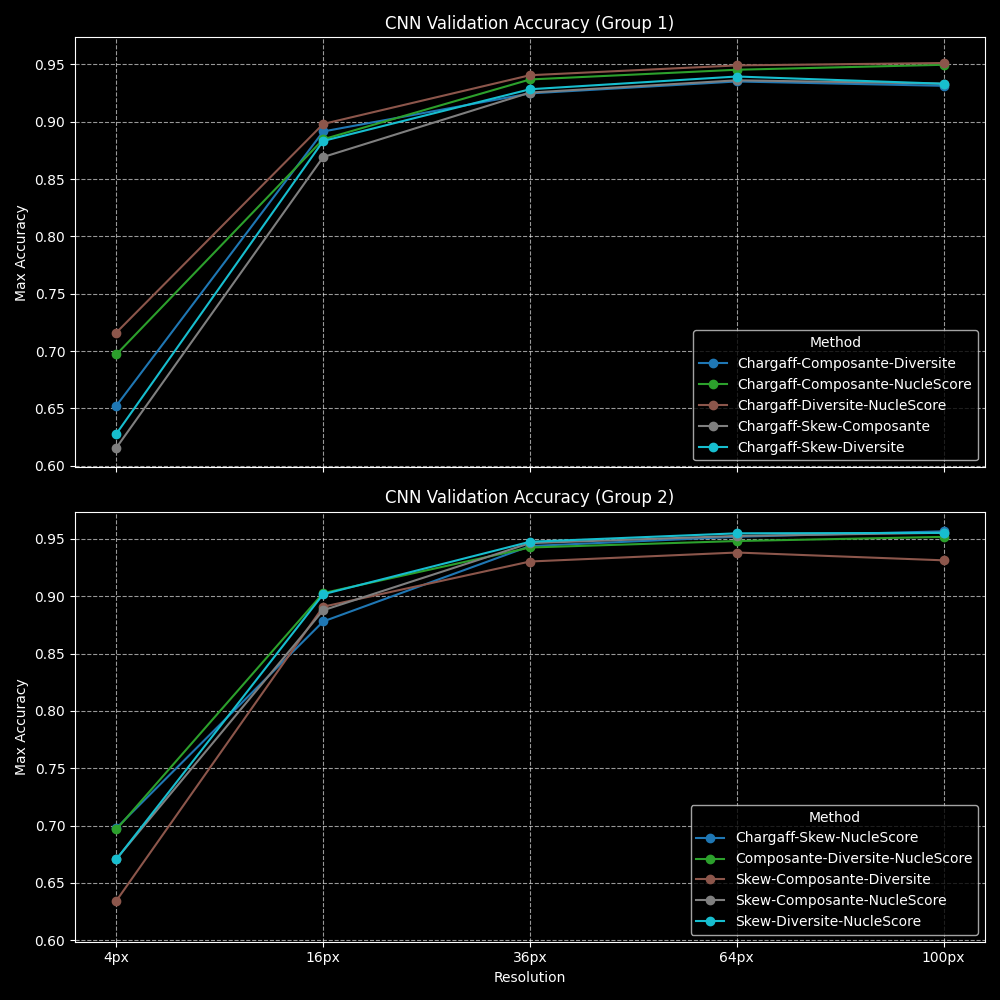
\includegraphics[width=0.7\textwidth]{../imgs/graphs/kfold/cnn_validation_accuracy_groups_mask_5_kfold_aug.png}
		\caption{Graph showing the validation accuracy of the CNN model with under-sampling applied on the different methods.}
		\label{fig:augmentation_accuracy}
	\end{figure}

	\begin{figure}[htbp!]
		\centering
		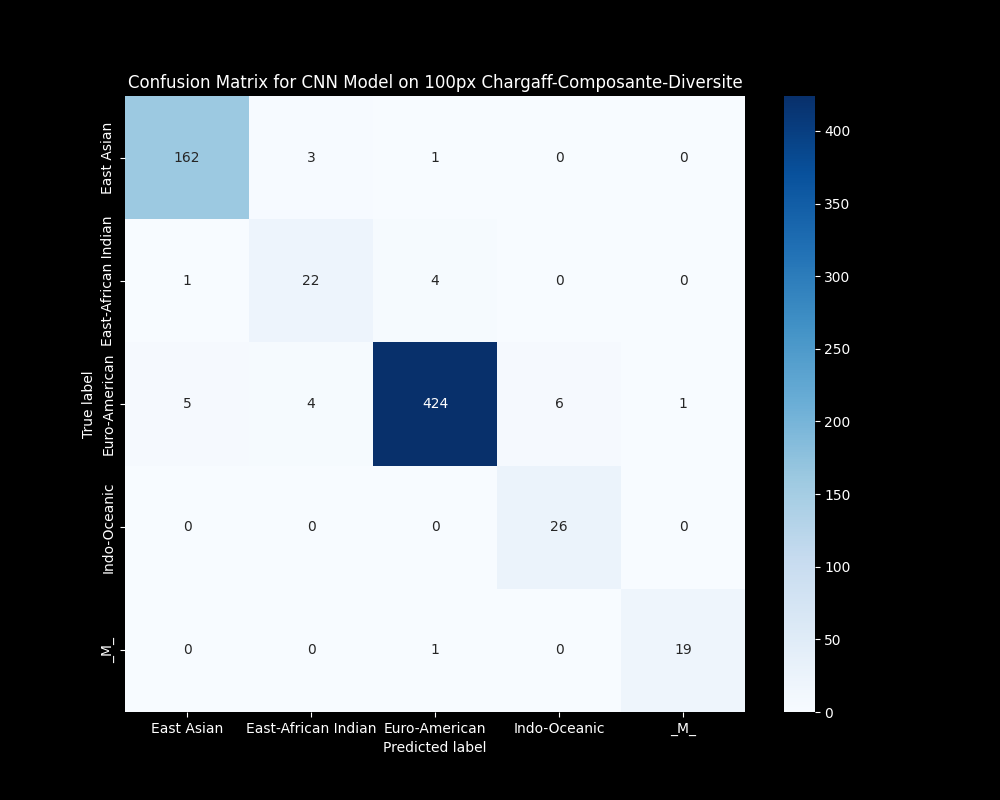
\includegraphics[width=0.7\textwidth]{../imgs/graphs/kfold/cnn_confusion_matrix_100px_mask_5-kfold_aug.png}
		\caption{Confusion matrix of the CNN model with under-sampling applied on the images obtained from the Chargaff-Diversity-NucleScore
			combination at 100px resolution.}
		\label{fig:augmentation_confusion_matrix}
	\end{figure}

	\begin{figure}[htbp!]
		\centering
		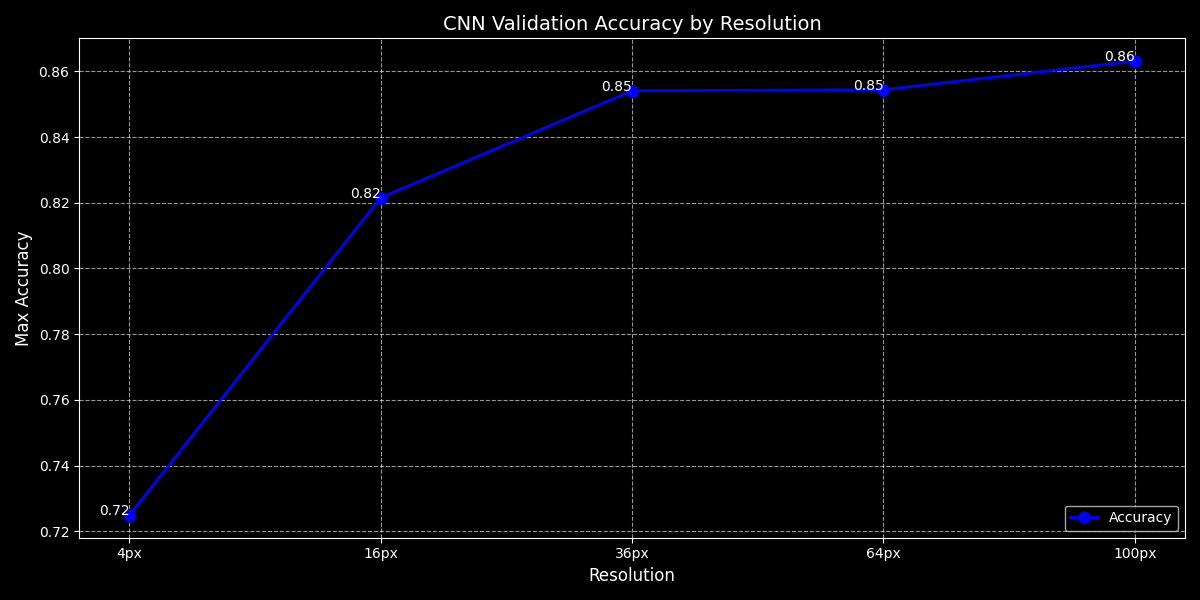
\includegraphics[width=0.7\textwidth]{../imgs/graphs/kfold/cnn_validation_accuracy_kfold_mosaics_line_mask_5_aug.png}
		\caption{Graph showing the validation accuracy of the CNN model with under-sampling applied on the mosaic images.}
		\label{fig:augmentation_accuracy_mosaic}
	\end{figure}

	\begin{figure}[htbp!]
		\centering
		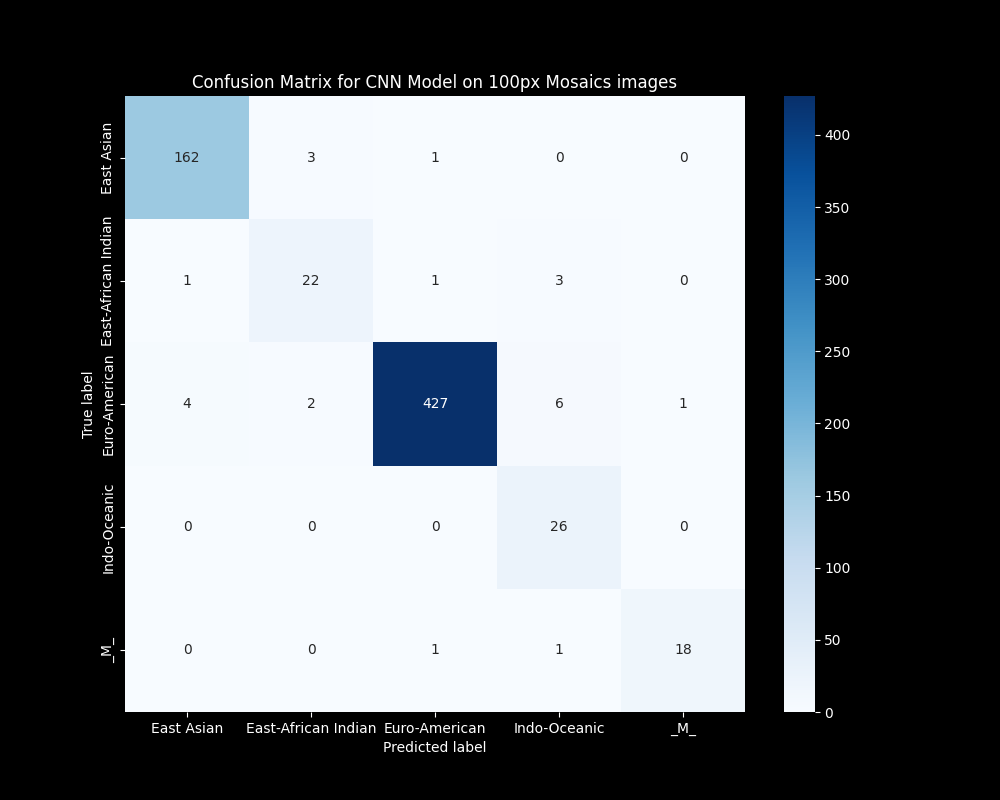
\includegraphics[width=0.7\textwidth]{../imgs/graphs/kfold/cnn_confusion_matrix_kfold_mosaics_100px_mask_5_aug.png}
		\caption{Confusion matrix of the CNN model with under-sampling applied on the mosaic images at 100px resolution.}
		\label{fig:augmentation_confusion_matrix_mosaic}
	\end{figure}

	% ------- kfold cross validation with combined techniques -------

	\begin{figure}[htbp!]
		\centering
		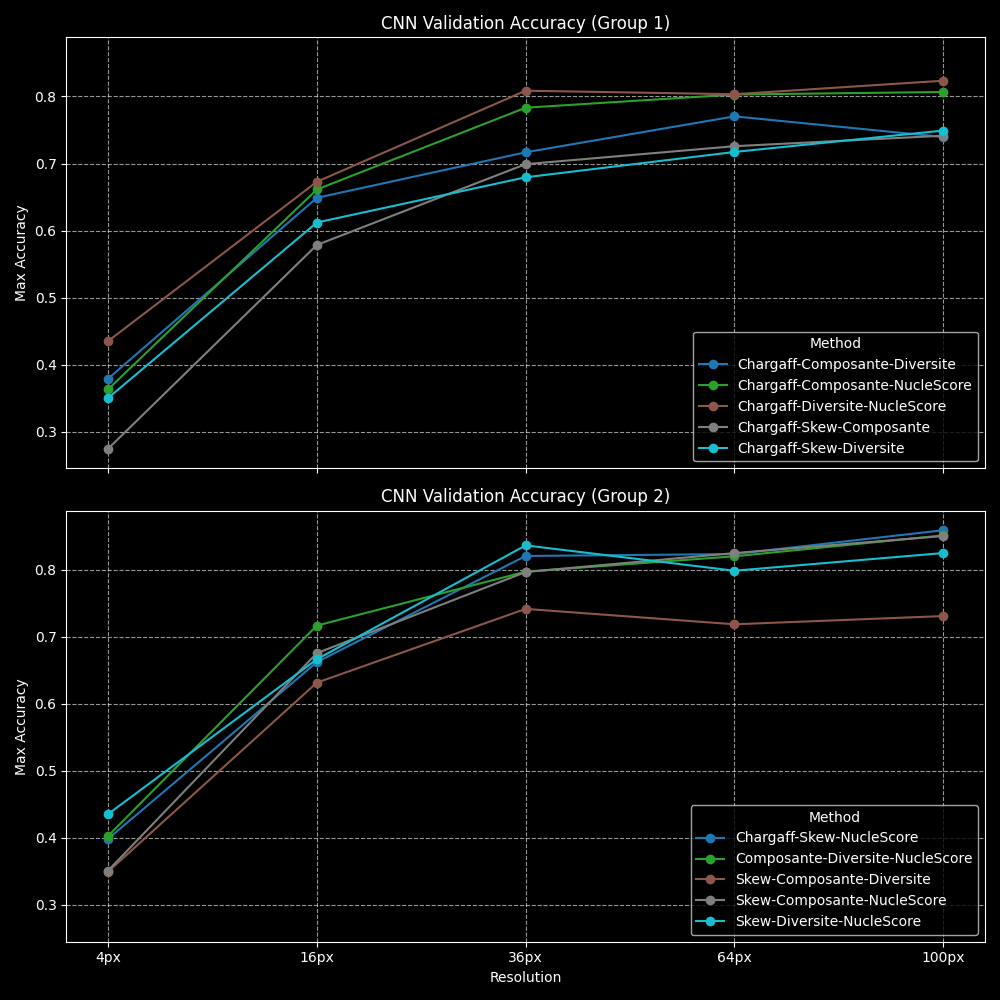
\includegraphics[width=0.7\textwidth]{../imgs/graphs/kfold-undersample/cnn_validation_accuracy_groups_mask_5_kfold_aug-under.png}
		\caption{Graph showing the validation accuracy of the CNN model with combined under-sampling and data augmentation
			techniques applied on the different methods.}
		\label{fig:combined_techniques_accuracy}
	\end{figure}

	\begin{figure}[htbp!]
		\centering
		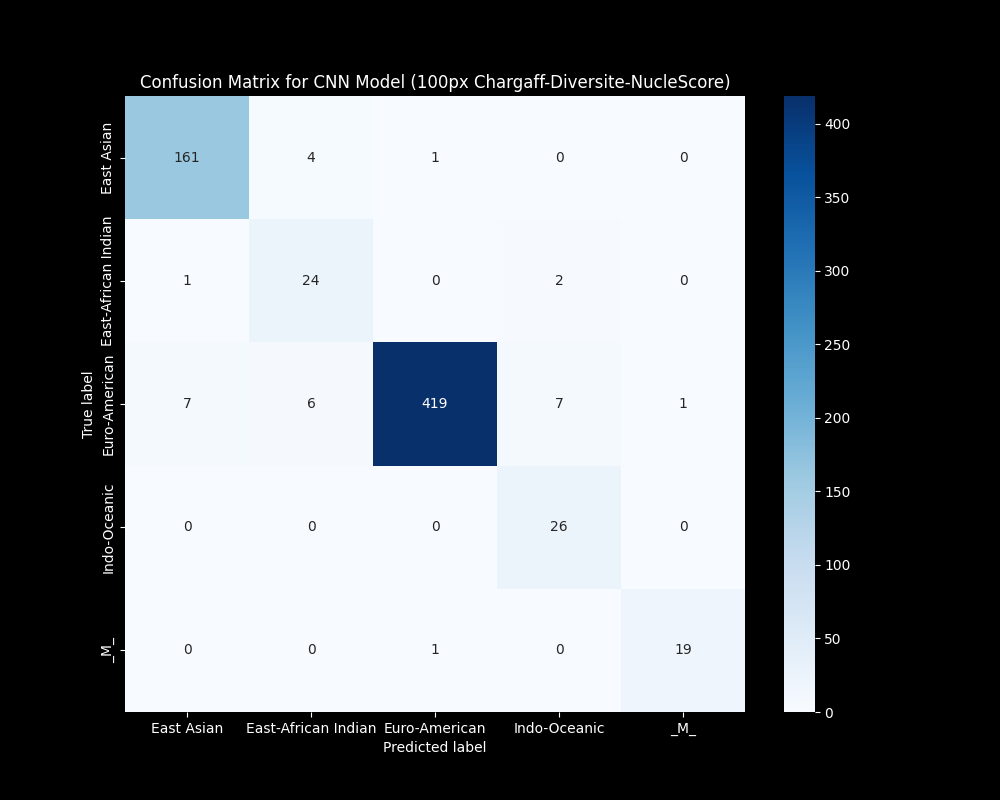
\includegraphics[width=0.7\textwidth]{../imgs/graphs/kfold-undersample/cnn_confusion_matrix_100px_mask_5-kfold_aug-under.png}
		\caption{Confusion matrix of the CNN model with combined under-sampling and data augmentation techniques
			applied on the images obtained from the Chargaff-Diversity-NucleScore combination at 100px resolution.}
		\label{fig:combined_techniques_confusion_matrix}
	\end{figure}

	\begin{figure}[htbp!]
		\centering
		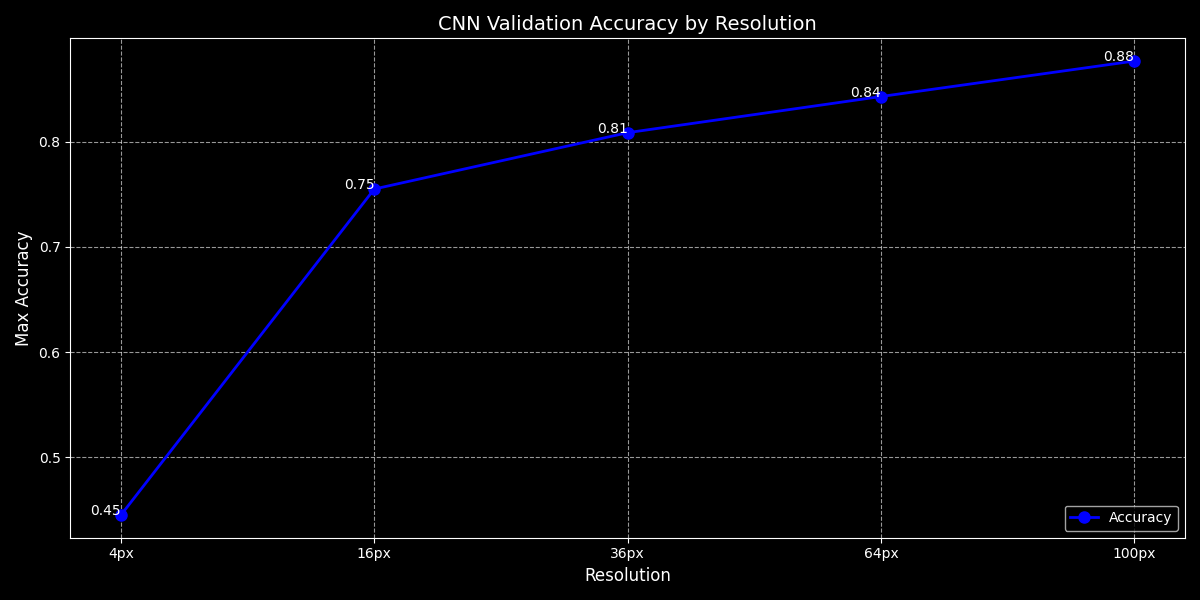
\includegraphics[width=0.7\textwidth]{../imgs/graphs/kfold-undersample/cnn_validation_accuracy_kfold_mosaics_line_mask_5_aug-under.png}
		\caption{Graph showing the validation accuracy of the CNN model with combined under-sampling and data augmentation
			techniques applied on the mosaic images.}
		\label{fig:combined_techniques_accuracy_mosaic}
	\end{figure}

	\begin{figure}[htbp!]
		\centering
		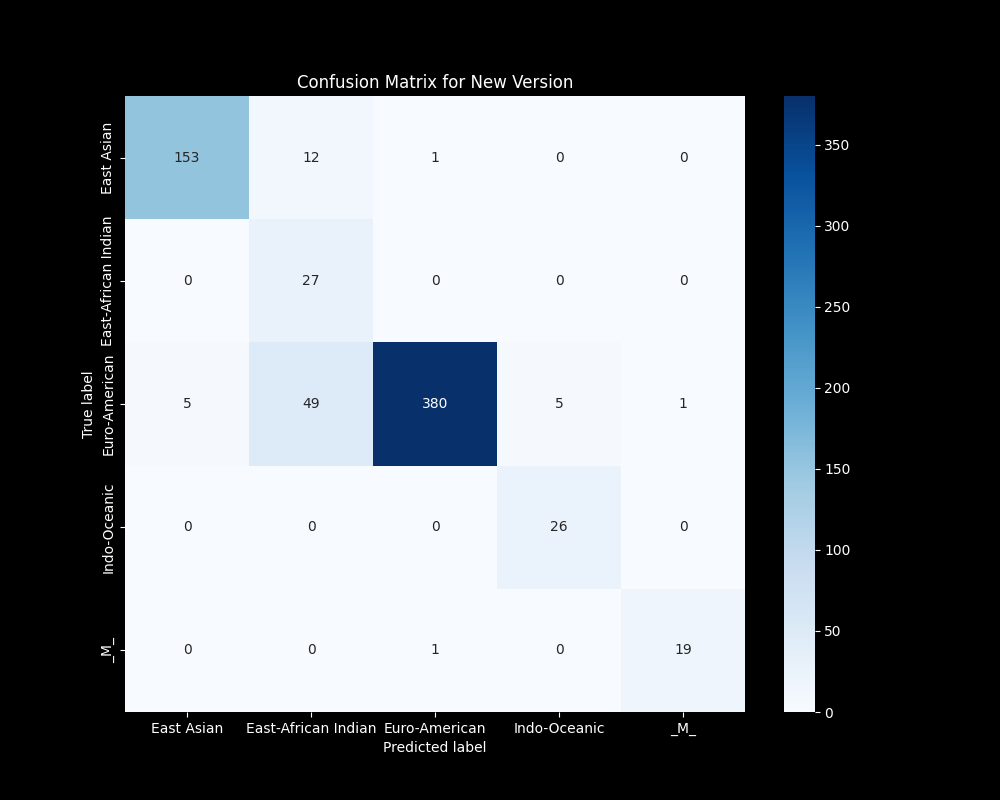
\includegraphics[width=0.7\textwidth]{../imgs/graphs/kfold-undersample/cnn_confusion_matrix_kfold_mosaics_100px_mask_5_aug-under.png}
		\caption{Confusion matrix of the CNN model with combined under-sampling and data augmentation techniques
			applied on the mosaic images at 100px resolution.}
		\label{fig:combined_techniques_confusion_matrix_mosaic}
	\end{figure}

\end{appendices}

\printbibliography
% \printbibliography[heading=subbibintoc,keyword={src},title={Data Sources}]

\end{document}